\documentclass{beamer}

\usetheme{Madrid}
\usecolortheme{beaver}

\usepackage[utf8]{inputenc}
\usepackage[brazil]{babel}
\usepackage{caption}
\usepackage{hyperref}
% \usepackage[style=abnt]{biblatex}
% \addbibresource{references.bib}
\usepackage{csquotes}

\title{Utilizando do Overleaf}
\author{Nightwind}
\institute[CTISM]{Colégio Técnico Industrial de Santa Maria}
\date{\today}

\begin{document}
    \frame{\titlepage}

    \begin{frame}
        \frametitle{Table of Contents}
        \tableofcontents
    \end{frame}

    \section[Página Inicial]{Página Inicial do Overleaf}
    \begin{frame}
        \frametitle{Homepage}
    \begin{figure}
        \centering
        \caption[HomePage]{Página Inicial do Overleaf.}
        \label{fig:homepageOverleaf}
        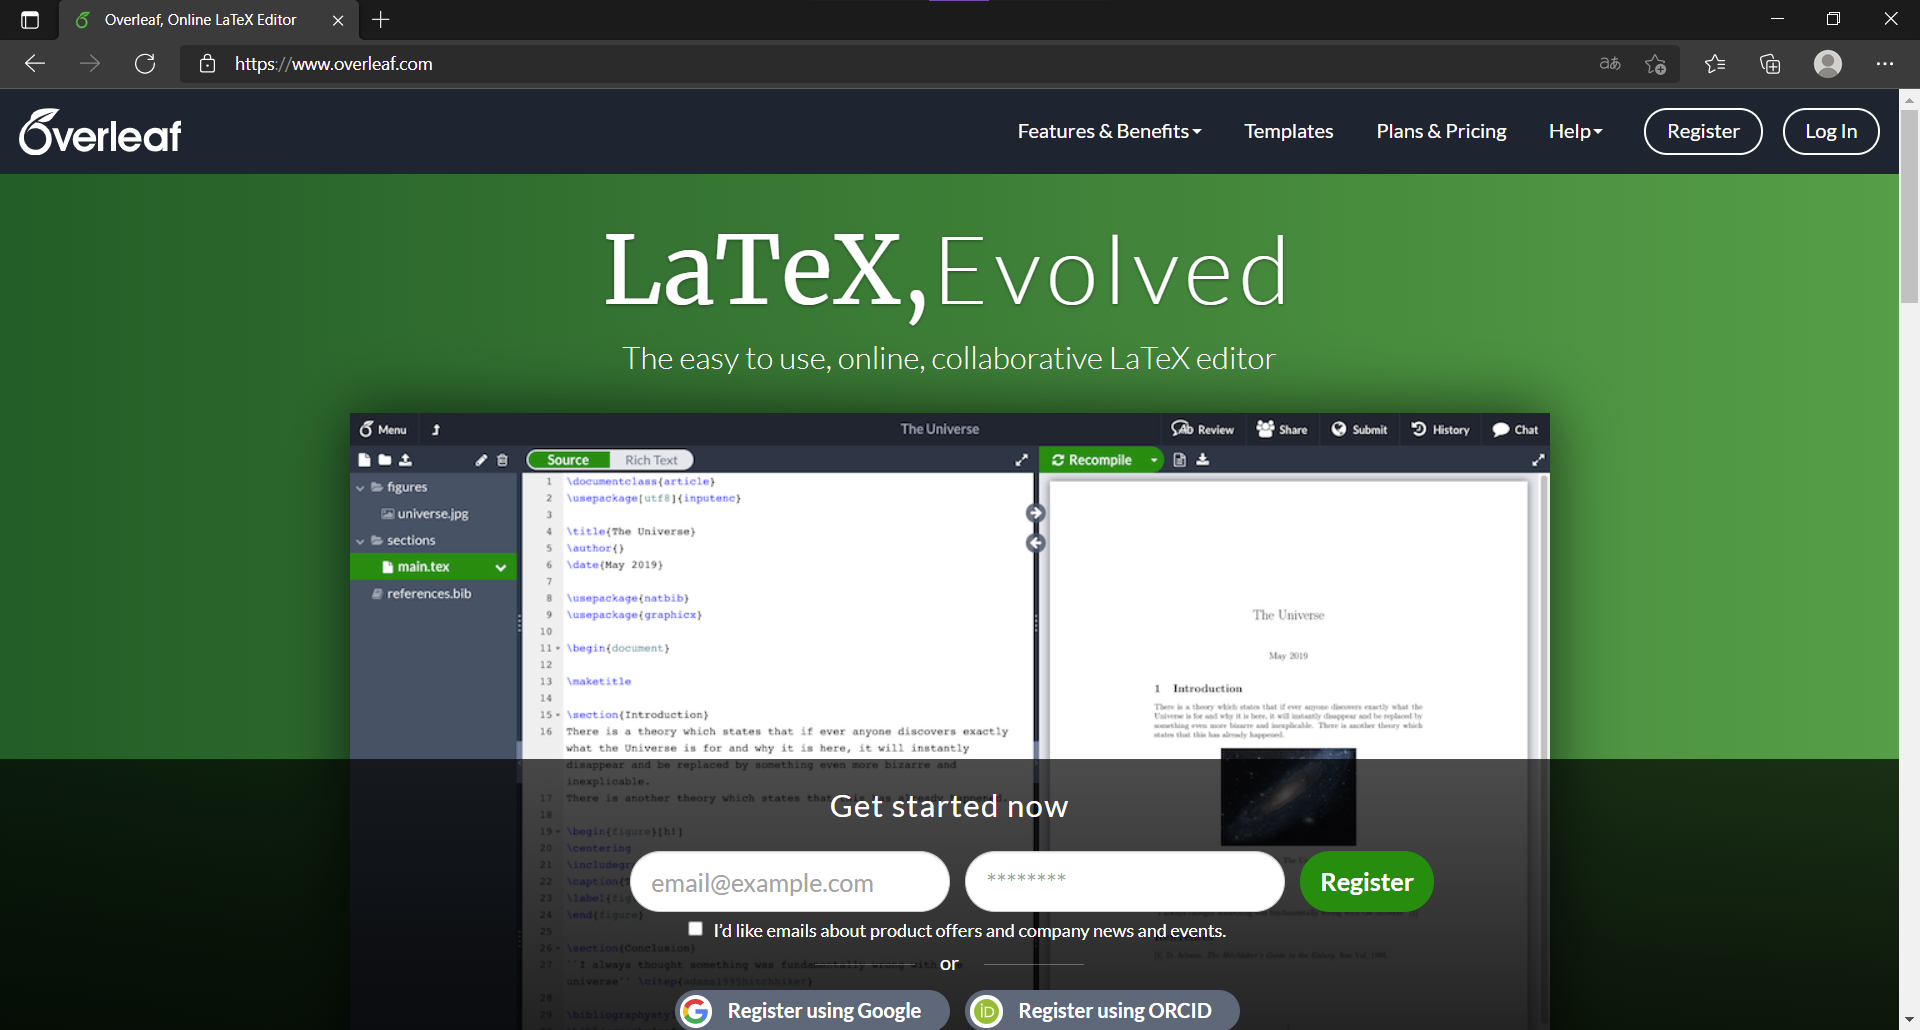
\includegraphics[width=0.9\textwidth]{../images/homepageOverleaf.png}
        \caption*{\footnotesize \url{https://www.overleaf.com/}}
    \end{figure}    
    \end{frame}

    \begin{frame}
        \frametitle{Homepage}
    \begin{itemize}
        \item Vá em ``\textit{Register}'' caso ainda não tenha uma conta.
        \item Vá em ``\textit{Log In}'' caso já tenha uma conta. 
        \item Coloque \textit{e-mail} e senha.
    \end{itemize}
        
    \section{Área do Usuário}
    \begin{frame}
        \frametitle{Novo usuário}
    \begin{figure}
        \centering
        \caption{Área do novo usuário.}
        \label{fig:newUserOverleaf}
        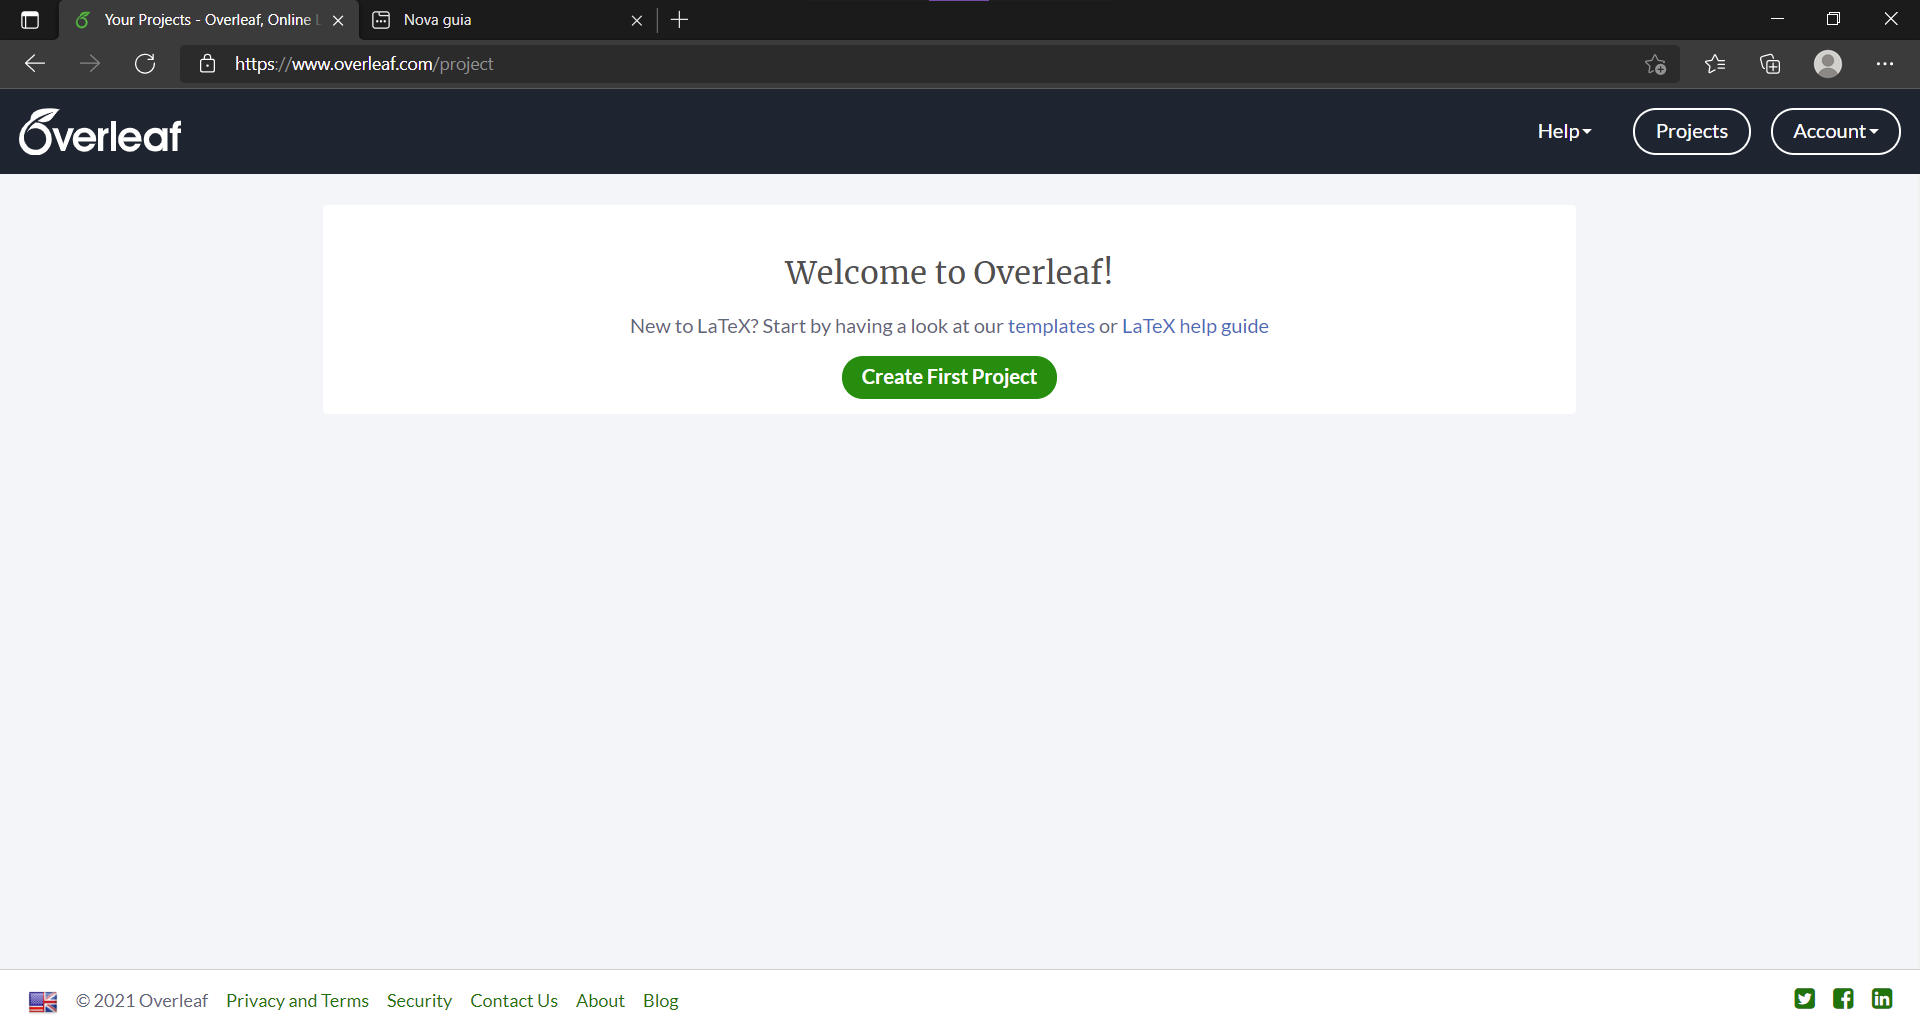
\includegraphics[width=0.9\textwidth]{../images/newUserOverleaf.png}
    \end{figure}
    \end{frame}

    \begin{frame}
        \frametitle{Novo usuário}
    \begin{itemize}
        \item teste
        % \item Para novos usuários, o \href{https://www.overleaf.com/}{Overleaf} recomenda visualizar os \href{https://www.overleaf.com/latex/templates}{Templates} e o \href{https://www.overleaf.com/learn}{Guia de \LaTeX}. Ambos são altamente recomendáveis. 
    \end{itemize}   
    \end{frame}

    % \begin{frame}
    %     \frametitle{Referencias}
    %     \printbibliography[type=online]{}
    % \end{frame}
\end{document}
